\section{Introduction}
\subsection{Real-World Relevance}
Charge is considered a fundamental property of matter. Even though multiple charged particles exist, in practice the electron is of greatest use in the field of electronics. Through the loss or gain of electrons, an electric charge is built-up and consequently, an electric field emerges. When placing a charge in an electric field, a force is applied to the charge. In consequence, when placing a travelling charge in an electric field, work is done upon the charge by the field\cite{Kammer2019}. Thus, a potential capable of producing a current arises, commonly called electricity. Over the past two decades, electricity has become essential in our day-to-day life. In the last 40 years alone, the net world wide yearly consumption of electricity has more than tripled, from \SI{7323}{\tera\W\hour} to \SI{23845}{\tera\W\hour}\cite{Alves2022}. Similarly, the access to electricity has increased from \SI{78.2}{\percent} to over \SI{90}{\percent} throughout the past 20 years alone\cite{WorldBank2020}. At this point, life without a large-scale electricity infrastructure would be inconceivable.

A battery is a device capable of storing electrical energy as chemical energy and releasing it in form of electricity\cite{Bates2012}. As the first effective storage medium for electricity, the battery is the foundation of modern portable electronics. Through the past 200 years, humanity has been perfecting the battery to supply evermore powerful devices with electricity\cite{Schumm2022}. Currently, nickel-metal-hybrid and lithium-ion technologies dominate the rechargeable-battery consumer market and are the second and third most used household batteries respectively\cite{Schumm2022}.\\
With the increase in sales of portable electronic devices, as shown in Fig. \ref{fig:smartphonesales}, as well as the increase in electric vehicle production and the recent surge towards renewable and eco-friendly energy engineering, the battery has become an essential foundation in many aspects of the modern lifestyle\cite{Laricchia2022,Tarascon2010,Relations2022}.
Particularly its use to counteract the inconsistent electricity production of renewable energy sources such as windfarms or solar panels, has given electrical energy storage a key role in the fight against global warming.

\begin{figure}[ht]
    \centering
    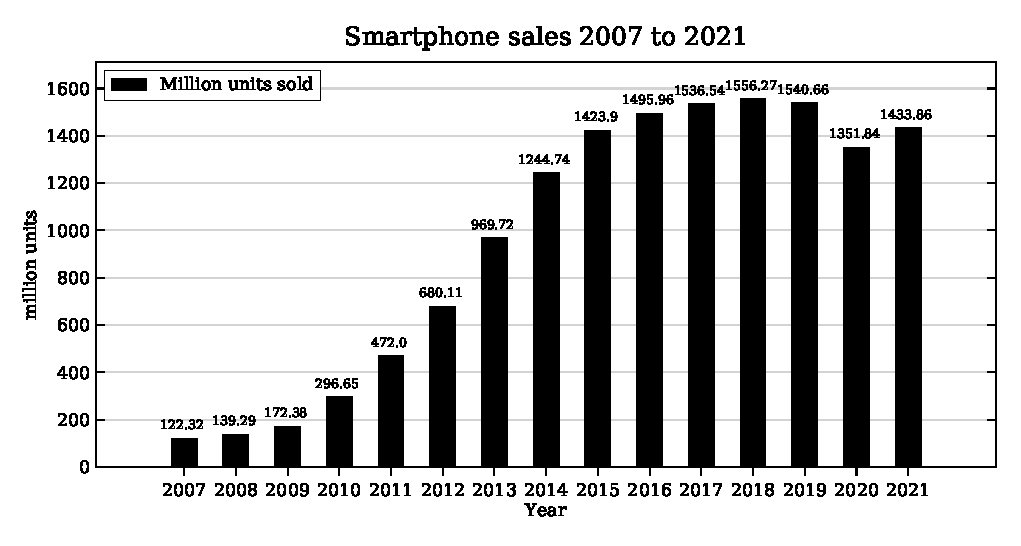
\includegraphics[width=\textwidth]{images/phonesales.eps}
    \caption{Number of smartphones sold to end users per annum from $2007$ to $2021$ in million units.}
    \label{fig:smartphonesales}
\end{figure}

\newpage

However, lithium-ion batteries are limited in multiple ways. Their construction promotes resource depletion and the release of poisonous substances into the environment \cite{Mrozik2021} - most notably, the use of rare metals such as cobalt, the estimated two million liters of water required for the mining of one metric ton of lithium, as well as the devastating impacts of toxic chemicals used for the extraction of lithium\cite{Katwala2018,Peters2017}. To prevent further pollution and help fight the global environmental crisis, more eco-friendly technologies are required. Sodium-ion batteries (SIBs) offer such a potential. Not only is sodium roughly 1000 times more naturally abundant than lithium, but its extraction also does not require harmful substances\cite{WikipediaAbun2022}. Furthermore, no rare metals are needed for the construction of sodium-ion batteries and their operation is less prone to thermal runaway\cite{Peters2016}. 

This investigation aims to assess the effectiveness and viability of homemade SIBs in the context of cost, safety, and environmental impact, while considering the production process as well as other state-of-the-art batteries.

\subsection{Investigation Context and Research Question}
The initial idea for the experiment is based on a sequence of videos published on YouTube\cite{Youtube2019}. They demonstrate the development of a solid-state sodium-ion battery constructed out of household materials over a period of multiple years. The core components include a graphite anode and a toothpaste cathode without an electrolyte and separator. However, these results were not reproducible. Furthermore, there was no research found to support these experiments. Most likely, the batteries seen in the videos are backed by years of experience and experimentation, which were non-replicable.

Thus, the scope of this investigation was adjusted to entail the construction of a sodium-ion battery and its evaluation in terms of viability and efficiency. Consequently, the following research question was chosen: To what extent are homemade sodium-ion batteries a viable and effective replacement for modern, state-of-the-art rechargeable batteries?.

Being restricted by the capabilities of a school laboratory, this experiment is unable to compete with cutting-edge research done around the world. However, since the core technology behind SIBs is comparatively simple, the focus was set on a more real-world relevant experiment. Based on instructions published by the University of Education in Freiburg, a simple sodium-ion accumulator is designed, constructed, and evaluated\cite{Klaus2022}. At its core, the battery consists of a titanium-dioxide layer applied to a fluorine-doped tin oxide (FTO) coated glass slide as a cathode, a graphite coated FTO glass slide as an anode and a sodium perchlorate solution as an electrolyte, based upon the instructions found online\cite{WikipediaFTO2022}.
FTO glass slides are chosen as current collectors to minimize the differences to a known, functional experiment and thus limit the sources of error. Further, titanium-dioxide and graphite are chosen, thanks to their ability to intercalate perchlorate ions and their use as both anodes and cathodes in previous works\cite{Guo2016}.
Due to substance limitations, the electrolyte was adapted, and de-ionized water is chosen, because of its use in aqueous sodium-ion batteries\cite{Che2017}. 
To evaluate the viability and efficiency, the battery's open circuit voltage, discharge curve and capacity are assessed and compared to a state-of-the-art lithium-ion battery by Panasonic\cite{Panasonic2018}. 
Furthermore, the process of construction, as well as the general state of knowledge concerning the field of sodium-ion batteries is taken into consideration.